\section{Evaluation}
\label{sec:evaluation}

\subsection{Benchmarks and conditions}
\label{sec:eval:benchmarks}
\label{sec:eval:conditions}
\label{sec:eval:ablations}

\textbf{$\tau^2$-bench retail}~\cite{tau2bench2025} is the
primary benchmark for the reader-side architecture head-to-head.
It scores state-validated pass$^k$ on a customer-service
tool-using domain.  We run $n{=}100$ tasks (seed 42), with Haiku
4.5 as both assistant and user simulator, a 20-turn budget, and
2 trials per task.  Cross-model and cross-domain probes
(\S\ref{sec:eval:results:sonnet}) use Sonnet 4.5 retail and
$\tau^2$-bench airline at $n{=}30$ each.

\subsection{Metrics and statistical methodology}
\label{sec:eval:metrics}
\label{sec:eval:stats}

\textbf{Completion rate} is the fraction of trials whose final
output passes the benchmark scorer.  \textbf{Pass$^k$} on
$\tau^2$-bench follows the unbiased estimator of Chen et al.: the
marginal success rate at $k{=}1$, and the both-trials-succeed
rate at $k{=}2$.  Two protocols are
\textbf{configuration-equivalent} at a given trial when code
inspection confirms identical request-side augmenter behavior at
that trial (system prompt prefix, tool-response modifications,
request headers, sampling parameters).  This is necessary but not
sufficient for byte-identical wire payloads
(\S\ref{sec:eval:request-equivalence}).

\textbf{Coordination-active pass$^k$
($\textsc{pass}^k_{\mathrm{active}}$)} restricts pass$^k$ to tasks
where the peer-coordination store is non-empty at each of trials
$1\!\ldots\!k$, the structurally-defined coordination-active
sub-event. It is causally pre-specifiable from the protocol
semantics: when the store is empty the coordination mechanism is
inactive, so any cross-protocol comparison on store-empty trials
measures noise rather than architecture. For $k{=}2$ in our
setting this is equivalently the trial-1 success rate on tasks
where trial~0 failed. Each contrast uses its own paired subset
(tasks where both compared protocols failed trial~0), so per-row
rates are not jointly comparable across contrasts.

Effect size throughout is Cliff's $\delta$ with the Romano et
al.\ (2006) magnitude thresholds. We apply paired sign tests
(binary pass$^k$ on $\tau^2$; the equivalent McNemar test agrees
and is reported in Table~\ref{tab:mde}). The $\tau^2$
head-to-head and coordination-active contrasts are reported
outside the Bonferroni correction families as the pre-specified
primary tests; all multiplicity corrections in this paper are
Bonferroni with $m{=}3$. All trials are logged to JSONL artifacts under
\texttt{eval/results/}; analysis is reproducible via the
\texttt{analysis} CLI in the repository.

\paragraph{Pre-registration.}  The Haiku $n{=}100$ retail
head-to-head is the pre-specified primary test: protocols,
$K{=}3$ writer, seed $42$, and $T{=}0$ were frozen before the run
($K{=}3$ was pilot-tuned on a prior $n{=}30$
sweep---\S\ref{sec:eval:limits}).
$\textsc{pass}^k_{\mathrm{active}}$ is causally pre-specifiable but
was applied to already-frozen data.  Sonnet, airline, M1, and P2
are exploratory; Sonnet $n{\geq}250$ retail is pre-registered as
confirmatory.

%==================================================================
% RESULTS
%==================================================================

\subsection{Results}
\label{sec:eval:results}

\subsubsection{Request-equivalence: what the trial-$0$ floor
measures}
\label{sec:eval:request-equivalence}

The trial-$0$ paired gap decomposes into four layered sources;
naming them keeps the headline numbers honest. The first is a
byte-identical first-request audit (E1); the second is
within-protocol API stochasticity at $\leq 3$\,pp (E2); the
third is between-protocol harness drift once the user-simulator
emits its first sampled output (E3); the fourth is a
hypothesized pull-specific structural perturbation (E4), which
the second seed did not confirm.
Strictly speaking, what we measure at trial $0$ is multi-turn
paired variance between two configuration-equivalent harness
runs; we label it a \emph{coordination noise floor} because it
is the gate any coordination claim on this benchmark must
clear, not because the variance itself is coordination-specific.
One structural consequence is worth making explicit: the floor
estimate is invariant to writer parameters such as $K$ by
construction. The writer fires only at the close of a trial with
reward $<1$, so no writer setting can perturb a trial-$0$
payload; $K$ shapes trial-$1$ coordination \emph{content}, and
its effects are diagnosed separately (M1--M3,
\S\ref{sec:eval:results:retail-intercept}).

At trial~$0$ the store is empty, so reader hooks are no-ops. The
three arms share the agent system prompt
(\texttt{AGENT\_SYSTEM\_TEMPLATE}; pull's augmenter returns input
unchanged when \texttt{warnings\_block()} is empty), the
protocol-independent tool list (no \texttt{trace.query}
injection), user-simulator prompt and priming, sampling parameters
(\texttt{T}{=}$0$, \texttt{max\_tokens}{=}$4096$, same
\texttt{claude-haiku-4-5}), and a pass-through intercept hook.
Two SHA-$256$ audits confirm E1: an offline reconstruction of
\texttt{client.messages.create} kwargs ($40/40$ cells
byte-identical: $n{=}10$ tasks $\times$ $4$ first-request
payload components, each hashed across all $3$ protocols) and a
live wire-byte audit ($30/30$ user-simulator opens
byte-identical on $10$ headline tasks).

The Messages API exposes no \texttt{seed}, so $T{=}0$ requests
are not bit-deterministic; a paired $n{=}30$ within-protocol
replicate (L3) bounds E2 at $\leq 3$\,pp. Once the user-simulator
emits its first sampled output, it becomes the agent's first
message and downstream wire bytes diverge across runs (within
\emph{or} between protocol); that drift is E3. Pull's
seed-$1$ $p_{\text{corr}}{=}0.012$ initially looked like a
small real structural perturbation in pull's augmenter (E4);
the second seed did not reproduce it (\S\ref{sec:eval:results:retail-intercept}),
so E4 is now a candidate-not-confirmed source rather than an
established one. E1--E3 together (plus E4 as a hypothesis) form
the \emph{configuration-equivalent} envelope, and the
coordination-active metric is designed to condition away E2--E4.
The head-to-head below measures any remaining effect against it.

\subsubsection{Reader-side architecture head-to-head: pull vs.\
intercept on $\tau^2$-bench retail}
\label{sec:eval:results:retail-intercept}

\textit{What this shows.} On the coordination-active subset
(trial~1 of tasks where trial~0 failed), pull and intercept tie
and both directionally underperform the no-coordination
baseline; with $n{=}8$--$17$ informative pairs after ties, the
subset is underpowered for a medium-sized effect, so we read
this as no detectable effect at this power rather than a clean
null. The trial-$0$ paired gaps anchor an empirical noise floor
that any architectural claim must clear. Pooled across two
$n{=}100$ seeds, the clean configuration-equivalent contrast
(no\_coord vs.\ intercept) gives $+5$\,pp (CI $[{-}2,{+}12]$,
not significant); the largest contrast (pull vs.\ intercept)
pools to $+7.5$\,pp with upper Wilson CI ${\approx}15$\,pp; and
the largest single-seed gap ($+18$\,pp, seed-$1$,
$p_{\text{corr}}{=}0.012$) did not reproduce at seed-$2$.

$\tau^2$-bench retail~\cite{tau2bench2025} reports state-validated
pass$^k$ on customer-service conversations
(\S\ref{sec:eval:benchmarks}). All runs use the
\textasciitilde$700$-line Anthropic-native harness
(\S\ref{sec:implementation}). A pilot $n{=}30$ smoke on the stock
$\tau^2$-bench/litellm pipeline observed $\geq30\%$ of Haiku 4.5
trials terminating with malformed
\texttt{tool\_use}/\texttt{tool\_result} sequences, silent at the
harness layer, consistent with the documented bug
class~\cite{litellmissue12404,litellmissue15322}. Our harness
observed zero infra errors across $600$ trials.

\paragraph{Protocols.}
The three protocols share an identical writer side.  At the close
of any trial with reward $<\!1$, the final $k{=}3$ tool calls
are written as \textsc{failed\_trial\_action} events in the
task-scoped store.  The $\tau^2$ harness uses this simplified
single event type instead of the full five-category taxonomy
of \S\ref{sec:arch:taxonomy} because retail trials
rarely surface explicit tool errors mid-trial; the failure signal
is the trial's terminal reward.  ($k{=}3$ is a causal-attribution
heuristic, pilot-tuned on a prior $n{=}30$ sweep; the $n{=}100$
run confirms this configuration rather than pre-registering
$k{=}3$ as optimal.)

The three protocols differ only in the reader interface.
\texttt{no\_coord} leaves the store unused. \texttt{pull}
(agent-as-reader) prepends a curated peer-warnings summary to the
agent's system prompt at trial start. \texttt{intercept}
(framework-as-reader) prepends a \texttt{[PEER-WARNING]} block to
the tool \emph{response} when the call's (name, arguments) match
a \textsc{failed\_trial\_action} event. Any pass$^k$ difference
between pull and intercept under matched payload is therefore
attributable to the reader-side architecture, and we observe none
at trial~1.

\paragraph{Setup and headline.}
100 tasks (seed 42) $\times$ 3 protocols $\times$ 2 trials gives
600 trials in total.  Both the assistant and the simulated user
are \texttt{claude-haiku-4-5} at $T{=}0$, with a 20-turn budget
per trial.  The task-scoped store is shared across the 2 trials
within a protocol cell.  Figure~\ref{fig:headline} summarizes the
result.  Table~\ref{tab:tau2retail:headline} reports cell-level
metrics; Table~\ref{tab:tau2retail:trial1} reports the
coordination-active paired tests.

\begin{table}[t]
\centering
\caption{$\tau^2$-bench retail headline results
($n=100$ tasks $\times$ 2 trials per protocol, 200 trials per
cell, Claude Haiku~4.5; zero infra errors across 600 trials).
All three protocols collapse to the same trial-1 success rate
($0.540$): coordination does not move the metric once the store
is populated.}
\label{tab:tau2retail:headline}
\small
\begin{tabular}{lrrrr}
\toprule
Protocol & succ.\ rate & pass$^1_{\mathrm{Chen}}$ & pass$^2_{\mathrm{Chen}}$ & Trial-1 succ.\ \\
\midrule
\texttt{no\_coord}  & 0.540 & 0.540 & 0.380 & 0.540 \\
\texttt{pull}       & 0.580 & 0.580 & 0.440 & 0.540 \\
\texttt{intercept}  & 0.490 & 0.490 & 0.330 & 0.540 \\
\bottomrule
\end{tabular}
\flushleft\footnotesize
Marginal cell metrics for the three protocols.
pass$^k_{\mathrm{Chen}}$ follows the Chen et al.\ unbiased
estimator (marginal success rate at $k{=}1$; both-trials-succeed
rate at $k{=}2$).  The \emph{trial-1 succ.\ rate} column reports
the success rate on trial~1 only, where the trace store contains
peer events from trial~0 and coordination is logically active.
\end{table}

\begin{table}[t]
\centering
\caption{Coordination-active pass$^k$ test (P4, defined in \S\ref{sec:eval:metrics};
\S\ref{sec:proposals}): paired sign tests on trial-1 outcomes
restricted to tasks where \emph{both} compared protocols had a
trial-0 failure, so both stores contain peer events and the
coordination mechanism is necessarily active.  Subset $n$ varies
by contrast.  All three pairwise comparisons fail to reject on
this subset; with $10/8/17$ informative pairs after ties the
test is underpowered for a medium-sized effect, so this is no
detectable effect at the available power rather than a clean
null.  The recovery-rate ordering against the \texttt{no\_coord}
baseline shows both coordination architectures slightly
underperforming no coordination at recovering from prior failure
(W/L/T = wins/losses/ties).}
\label{tab:tau2retail:trial1}
\small
\begin{tabular}{lrcrr}
\toprule
Comparison & subset $n$ & t1 succ.\ rate & W/L/T & sign $p$ \\
\midrule
pull vs.\ intercept & 29 & 0.28 / 0.28 & 5 / 5 / 19 & $1.00$ \\
pull vs.\ no\_coord & 28 & 0.14 / 0.29 & 2 / 6 / 20 & $0.29$ \\
intercept vs.\ no\_coord & 35 & 0.20 / 0.34 & 6 / 11 / 18 & $0.33$ \\
\bottomrule
\end{tabular}
\flushleft\footnotesize
Each contrast uses its own paired subset; rows are not
cross-comparable.  The high tie counts ($19$, $20$, $18$) leave
informative samples of $10$, $8$, $17$ tasks, so these sign
tests are near-powerless and the directional recovery deficits
are hypothesis-generating only.  Unconditional trial-1 paired
sign tests over all $n{=}100$ tasks return identical ties
(pull-vs-intercept $13/13/74$; pull-vs-no\_coord $19/19/62$;
intercept-vs-no\_coord $20/20/60$; all $p{=}1.0$).  This table
conditions on trial-0 failure; the pass$^2$ column in
Table~\ref{tab:tau2retail:headline} counts both-trials-success
unconditionally over all 100 tasks.  The two are arithmetically
consistent: pull's pass$^2{=}0.44$ equals $0.71 \times 62/100$,
where $0.71$ is pull's conditional trial-1 success rate given
trial-0 success.
\end{table}

\paragraph{Coordination-active head-to-head: no detectable
effect at this power.}
The trial-1 outcome on the trial-0-failed subset was pre-specified
as the architectural test (P4; \S\ref{sec:eval:metrics}): on those
tasks the store contains peer events, so the coordination
mechanism is active. Pull and intercept tie at trial-1 success
rate $0.28$ on the 29-task both-failed subset (paired sign test
$W/L/T=5/5/19$, $p=1.0$). Each directionally underperforms
\texttt{no\_coord} on its own trial-0-failed subset (pull $0.143$
vs.\ $0.286$, $n{=}28$; intercept $0.20$ vs.\ $0.343$, $n{=}35$),
but neither reaches significance at this subset size. After
ties, the informative pairs number $10/8/17$, well below the
power needed to detect a medium-sized effect; ``null'' would
overclaim, and we read this as no detectable effect at the
available power rather than evidence that the mechanisms are
inert. The unconditional trial-$1$ test over all 100 tasks
returns identical ties. The takeaway is that the naive
deployed-today coordination forms (last-$K$ writers paired with
either curated reading or per-match injection) do not transfer
peer state into pass$^k$ at this scale and model, and the
directional evidence is at least consistent with mild
interference rather than help; both readings would require a
larger paired sample to separate.

\paragraph{Trial-0 decomposition: an empirical noise-floor estimate.}
At trial~0 the store is empty under every protocol, so the
coordination mechanism is inactive. Of the three pairwise
contrasts, only no\_coord-vs-intercept is genuinely
configuration-equivalent: code inspection (see
\texttt{protocols.py}) confirms that both arms reduce to
pure no-ops on the empty store. Pull's reader still re-enters
its augmenter on every trial-$0$ turn (which returns input
unchanged when \texttt{warnings\_block()} is empty), so its
contrast with the other two arms is not configuration-equivalent
in the same sense, so its contrasts must be read separately
from the clean one.
Paired sign tests at seed-$1$ ($n{=}100$, Bonferroni $m{=}3$;
the second seed follows below):
no\_coord-vs-intercept $21/11/68$
($p_{\text{corr}}{=}0.330$); pull-vs-no\_coord $18/10/72$
($p_{\text{corr}}{=}0.555$); pull-vs-intercept $27/9/64$
($p_{\text{corr}}{=}0.012$). Wilson $95\%$ CIs on the signed
gaps are $[{-}2,{+}16]$\,pp, $[{-}1,{+}19]$\,pp, and $[{+}6,{+}26]$\,pp
respectively: the first two cross zero, the third does not---at
this seed.

\paragraph{Reproducibility: a second seed.}
We re-ran the full $n{=}100$ retail sweep at a second seed
(\texttt{seed42$\to$seed-2}, same task IDs, same harness, fresh
API draws). Trial-$1$ rates remain effectively flat
($0.520/0.540/0.510$ for no\_coord/pull/intercept); the
head-to-head still shows no detectable effect. Trial-$0$ paired
sign tests at seed-$2$: no\_coord-vs-intercept $13/13/74$
($0$\,pp signed gap, $p_{\text{corr}}{=}1.0$); pull-vs-no\_coord
$15/18/67$ ($-3$\,pp, $p_{\text{corr}}{=}1.0$);
\textbf{pull-vs-intercept $18/21/61$
($-3$\,pp, $p_{\text{corr}}{=}1.0$)}.  The seed-$1$ $+18$\,pp
pull-vs-intercept significance does not reproduce; the sign
even flips. We correspondingly retract E4 (pull-specific
structural perturbation) as an established finding---a single
seed's $p_{\text{corr}}{=}0.012$ on a contrast that pools to
$45/30/125$ ($+7.5$\,pp, $p_{\text{corr}}{=}0.316$) over both
seeds is exactly the artifact a paired noise-floor protocol
should catch, and ours did.

Pooled across both seeds ($n{=}200$): no\_coord-vs-intercept
$34/24/142$ ($+5$\,pp, CI $[{-}2,{+}12]$\,pp,
$p_{\text{corr}}{=}0.711$); pull-vs-no\_coord $33/28/139$
($+2.5$\,pp, $p_{\text{corr}}{=}1.0$); pull-vs-intercept
$45/30/125$ ($+7.5$\,pp, CI $[{-}1,{+}15]$\,pp,
$p_{\text{corr}}{=}0.316$). \emph{No paired contrast is
significant after Bonferroni at any single seed or pooled.}
The clean-contrast pooled signed gap is $\approx 5$\,pp with
Wilson upper bound $\sim 12$\,pp; the largest pooled upper bound
across any contrast is $\sim 15$\,pp (pull-vs-intercept). The
across-seed observed range of signed gaps is
$[{-}3,{+}18]$\,pp, with the upper end anchored on a single
seed that did not replicate. We therefore characterize the
configuration-equivalent floor as a paired-disagreement
envelope whose pooled upper CI is $\lesssim 15$\,pp; calling
it ``10--18\,pp'' from one seed alone overclaimed the
precision. The motivation for P4 (coordination-active
pass$^k$, \S\ref{sec:eval:metrics}) stands: even a
${\sim}15$\,pp envelope swamps the small headline gains
recent coordination architectures report.

\paragraph{Mechanism diagnosis: three failure modes.}
\emph{(M1) Writer mis-attribution.} The causally-relevant call is
often upstream; last-$K$ records downstream symptoms. A
single-judge Haiku 4.5 LLM-judge audit on $30$ analyzable
trial-$0$ failures returns $77\%$ \textsc{upstream}
(direction-of-magnitude motivation, not a confirmed effect; see
L4 in \S\ref{sec:eval:limits}).
\emph{(M2) Per-match injection noise.} The intercept store
accumulates $\bar{n}{=}2.77$ events per trial (max $8$), and each
matching call fires a separate warning.
\emph{(M3) Brittle keying.} Literal-tuple payloads do not
transfer: \texttt{cancel\_order(\#W123)} does not match
\texttt{cancel\_order(\#W456)} even when both target shipped
orders. \S\ref{sec:proposals} discusses refinements matched
to M1--M3.

\begin{figure*}[t]
\centering
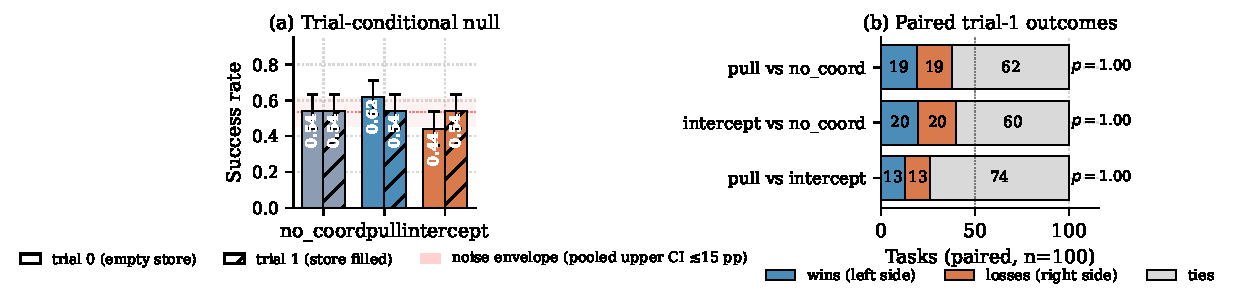
\includegraphics[width=0.84\textwidth]{figures/fig_combined.pdf}
\caption{Headline visual (seed-$1$ of two $n{=}100$ seeds;
\S\ref{sec:eval:results:retail-intercept} reports the second
seed and pooled tests). The coordination-active head-to-head
shows no detectable effect at the available power; the trial-$0$
paired gap is the noise-floor estimate.
\textbf{(a) Coordination-active head-to-head.}  Success rate by
protocol at trial~0 (empty store, coordination inert) and
trial~1 (store filled).  \texttt{no\_coord} and intercept are
configuration-equivalent at trial~0 by code inspection; their
$+10$\,pp signed paired gap at this seed (Bonferroni
$p_{\text{corr}}{=}0.330$, CI $[{-}2,{+}16]$ crosses zero)
pools to $+5$\,pp (CI $[{-}2,{+}12]$) across both seeds and is
the clean empirical noise floor. Pull's $+18$\,pp paired gap
against intercept at this seed ($p_{\text{corr}}{=}0.012$) did
not reproduce at seed-$2$ ($-3$\,pp, $p_{\text{corr}}{=}1.0$;
pooled $+7.5$\,pp, upper CI ${\approx}15$\,pp), so we read it
as a single-seed draw from the envelope rather than an
established pull-specific perturbation. At trial~1, where
coordination is logically active, all
three protocols collapse to $0.54$.
\textbf{(b) Paired trial-1 outcomes} over $n{=}100$ tasks.  Ties
dominate; all three sign tests fail to reject the no-difference
null ($p{=}1.0$). Informative pairs after ties on the
coordination-active subsets of
Table~\ref{tab:tau2retail:trial1} are $10/8/17$, so this is no
detectable effect at the available power rather than a clean
null.}
\label{fig:headline}
\Description{Two-panel figure. Panel (a) is a grouped bar chart of
success rate (trial 0 vs trial 1) for no_coord, pull, intercept;
trial 1 is flat at 0.54 for all three. Panel (b) is a horizontal
stacked bar chart of wins/losses/ties for the three pairwise
contrasts; ties dominate.}
\end{figure*}

\subsection{Cross-model and cross-domain probes}
\label{sec:eval:results:sonnet}
\label{sec:eval:results:airline}

\begin{figure*}[t]
\centering
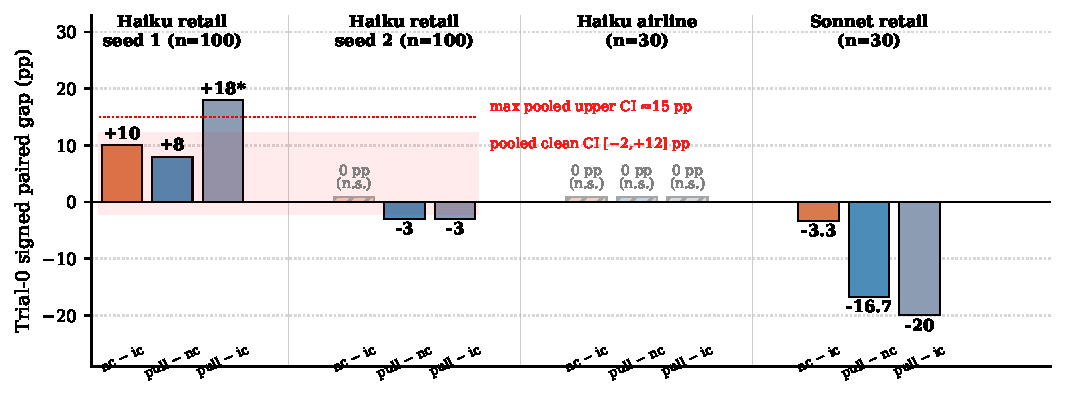
\includegraphics[width=0.92\textwidth]{figures/fig_noise_floor.pdf}
\caption{Trial-0 paired-sign-test signed gaps across seed,
model, domain, and contrast. The noise floor is a measurement
output of the coordination-active pass$^k$ protocol, not a
universal constant. Haiku retail: the seed-$1$ gaps
($+10/{+}8/{+}18$\,pp) collapse to $0/{-}3/{-}3$\,pp at
seed-$2$; the red band marks the pooled clean-contrast CI
$[{-}2,{+}12]$\,pp and the dotted line the largest pooled upper
Wilson CI ${\approx}15$\,pp. The starred seed-$1$ $+18$\,pp bar
is the non-replicating single-seed result retracted in
\S\ref{sec:eval:results:retail-intercept}. The floor is domain-
and capability-dependent: Haiku airline at $n{=}30$ shows
$0$\,pp gaps across all three contrasts, while Sonnet retail at
$n{=}30$ spans magnitudes $3.3$--$20$\,pp with the direction
flipped---pull starts trial-0 \emph{behind} \texttt{no\_coord}
on Sonnet rather than ahead---so the $20$\,pp magnitude there
sits slightly above the upper edge of the Haiku-retail
observations.}
\label{fig:noise-floor}
\Description{Bar chart of signed trial-0 paired gaps in four
groups. Haiku retail seed 1 at +10/+8/+18pp; Haiku retail seed
2 at 0/-3/-3pp; Haiku airline at 0pp; Sonnet retail at
-3.3/-16.7/-20pp. Red band marks the pooled clean-contrast CI
[-2,+12]pp over the two Haiku retail groups, with a dotted line
at the +15pp largest pooled upper CI.}
\end{figure*}

Two $n{=}30$ probes test whether the underpowered non-result
and the floor are Haiku-retail-specific;
Figure~\ref{fig:noise-floor} summarizes the trial-$0$ gaps.
The probes illustrate the metric rather than making
coordination claims at this scale.

\paragraph{Sonnet 4.5 retail $n{=}30$.}
Trial-1 rates: \texttt{no\_coord} $0.500$, pull $0.733$,
intercept $0.733$; raw pull-vs-no\_coord $p{=}0.039$ does not
survive Bonferroni $m{=}3$. The trial-$0$ gap magnitudes span
$3.3$--$20$\,pp (overlapping the Haiku-retail observations,
with the largest magnitude slightly above their upper edge)
but with the direction flipped: pull starts $-16.7$\,pp
\emph{behind} at trial~$0$, so its $+23$\,pp marginal gain partly
recovers an unrelated trial-$0$ deficit. The coordination-active
metric makes this direction-flip visible; marginal pass$^1$
obscures it. Sonnet $n{\geq}250$ is pre-registered as
confirmatory.

\paragraph{Haiku airline $n{=}30$.}
Trial-1 rates: \texttt{no\_coord} $0.500$, pull $0.533$,
intercept $0.567$ (all paired $p{>}0.69$); trial-0 gaps collapse
to $\approx 0$\,pp, so the floor is domain-dependent. On the
coordination-active subset ($n{=}14$), the direction matches
retail (\texttt{no\_coord} $0.357$, intercept $0.286$, pull
$0.214$): the naive last-$K$ scheme does not help and plausibly
impairs recovery.

\subsection{From noise floor to deployment threshold}
\label{sec:eval:deployment}

Converted to a release-time decision rule, the Haiku-retail
envelope (pooled upper Wilson CI ${\approx}15$\,pp,
\S\ref{sec:eval:results:retail-intercept}) becomes a
\emph{minimum detectable effect (MDE)} for sample-size planning
within that regime. Because the floor varies by domain (Haiku
airline $\approx 0$\,pp) and capability tier (Sonnet retail
magnitudes $3.3$--$20$\,pp), the MDE table is regime-specific, and transport
to other model/domain pairs requires re-running the paired
protocol. Applying a two-proportion $z$-test at $\alpha{=}0.05$,
power $0.80$, baseline $p_1{=}0.50$, Table~\ref{tab:mde} gives
the required sample sizes.

\paragraph{What transfers, and a cheap probe.}
Re-running the full paired protocol per (model, domain) pair is
the gold standard but not the entry cost. The floor's observed
variation tracks two identifiable drivers: how much of the task
set sits near the model's decision boundary (Haiku airline
collapses to $0$\,pp gaps because most trial-$0$ outcomes are
ties; Sonnet retail shifts which tasks are marginal, flipping
gap direction), and the user-simulator's sampled-output entropy,
which seeds the E3 drift. Both are estimable from a paired
$n{=}30$ clean-contrast probe (baseline vs.\ an inert-hooked
baseline) before any full sweep: our own $n{=}30$ probes are
what surfaced the airline collapse and the Sonnet direction
flip. The practical rule we propose: report a same-model paired
probe alongside any coordination claim, and escalate to the
full $n{\geq}100$ protocol only when the claimed effect is
within ${\sim}2\times$ the probe's upper CI.

\begin{table}[t]
\centering
\caption{Minimum sample size (tasks per arm) to detect a
candidate pass$^k$ improvement $\Delta$ on $\tau^2$-bench retail
at $\alpha{=}0.05$, power $0.80$, baseline $p_1{=}0.50$.
``Indep.'' is the two-proportion $z$-test for independent arms.
``Paired'' is the McNemar test calibrated on the seed-$1$
trial-0 discordance rate ($p_d{=}0.32$, \texttt{no\_coord} vs.\
intercept; pooled across both seeds $p_d{=}0.29$, which barely
moves the column).  Read-out: $\tau^2$-bench retail's public
114 tasks at one seed detect only $\Delta{\geq}20$\,pp at the
independent-arm rate ($n{=}93$), or $\Delta{\geq}15$\,pp
paired ($n{=}110$).}
\label{tab:mde}
\small
\begin{tabular}{rrrr}
\toprule
$\Delta$ (pp) & Indep.\ $n$ & Paired $n$ & $\tau^2$-retail seeds$^\ast$ \\
\midrule
5  & 1565 & 1003 & impractical \\
10 & 388  & 249  & 4 seeds / 3 paired \\
\textbf{15} & \textbf{170}  & \textbf{110}  & \textbf{2 seeds / 1 paired} \\
18 & 117  & 76   & 2 seeds / 1 paired \\
20 & 93   & 61   & 1 seed / 1 paired \\
25 & 58   & 38   & 1 seed / 1 paired \\
\bottomrule
\end{tabular}
\flushleft\footnotesize
$^\ast$ Number of full $114$-task seeds required to reach $n$;
``paired'' counts the paired condition.
\end{table}

\paragraph{Motivation only: literature gap-size context.}
Table~\ref{tab:literature-vs-floor} sets ten recent multi-agent
coordination contributions next to the Haiku-retail pooled
envelope: seven headline gains fall below the clean-contrast
pooled upper CI ($12$\,pp) and one more sits inside the
$12$--$15$\,pp band up to the largest pooled upper CI. The ten are recent (2023--2026) multi-agent
coordination architecture papers we found citing
MAST~\cite{mast2025} or CodeDelegator~\cite{codedelegator2026}
and reporting a single-number headline architectural delta on a
named benchmark; this is illustrative rather than systematic.
The point is to motivate reporting same-model paired floors
alongside future coordination claims, not to adjudicate the
underlying systems in their original (different model, task,
metric, $n$) settings, which would require per-row paired
replication. We acknowledge the tension head-on: this paper
argues against single-number cross-setting comparisons, and
Table~\ref{tab:literature-vs-floor} is precisely that
juxtaposition; we include it as a motivating prompt because
the gap-size visibility outweighs the methodological cost,
not because the comparison itself adjudicates anything.

\begin{table}[t]
\centering
\caption{Motivation examples for why same-model paired floors
matter; not a verdict on the underlying systems. Each row's
effect is shown alongside our Haiku-retail pooled envelope
purely to motivate the protocol; the comparison is heterogeneous
(different model, task, metric, $n$) and any individual row may
be entirely real in its original setting. ``vs.\ floor'' marks
whether the published gap is below the clean-contrast pooled
upper CI of $12$\,pp ($\downarrow$), inside the $12$--$15$\,pp
band up to the largest pooled upper CI ($=$), or above
$15$\,pp ($\uparrow$); the floor itself varies by model
and domain (\S\ref{sec:eval:results:airline}). Read $\downarrow$
as \emph{unresolved against a same-setting paired floor}, never
as \emph{refuted}.}
\label{tab:literature-vs-floor}
\small
\setlength{\tabcolsep}{4pt}
\begin{tabular}{lll@{\hspace{6pt}}c}
\toprule
Paper & Bench / Task & Effect & vs.\ floor \\
\midrule
CA-MCP~\cite{camcp2026}            & TravelPlanner BERTScore & $+1.2$ pts & $\downarrow$ \\
Terrarium~\cite{terrarium2025}     & Meeting Scheduling      & $1.0$--$2.7$\,pp & $\downarrow$ \\
AgentVerse~\cite{agentverse2023}   & HumanEval (Solo vs.\ Group)  & $+1.8$\,pp  & $\downarrow$ \\
AutoGen~\cite{autogen2023}         & MathChat over PoT/PS    & $\sim$$+6$\,pp & $\downarrow$ \\
MetaGPT~\cite{metagpt2024}         & SoftwareDev quality     & $<10$\,pp & $\downarrow$ \\
Silo-Bench~\cite{silobench2026}    & GPT-OSS P2P vs.\ BP     & $+6$\,pp & $\downarrow$ \\
Reflexion~\cite{reflexion2023}     & HumanEval                  & $+11$\,pp   & $\downarrow$ \\
\midrule
Ou et al.~\cite{ou2025coordination} & TravelPlanner orch.+notebook & $+13.5$\,pp & $=$ \\
\midrule
Reflexion~\cite{reflexion2023}     & ALFWorld                    & $+22$\,pp & $\uparrow$ \\
Ou et al.~\cite{ou2025coordination} & TravelPlanner combined     & $+17.5$\,pp & $\uparrow$ \\
\bottomrule
\end{tabular}
\end{table}

Coordination-active pass$^k$ is the minimum pre-deployment
measurement gate that any coordination claim on $\tau^2$-bench
(and the broader $\tau$-bench family of state-validated
benchmarks) should pass; Table~\ref{tab:mde} ships the
release-gate.

\paragraph{Monitoring schema.}
Three runtime rules for AgentCore / SageMaker Model
Monitor~\cite{sagemaker_monitor2022} deployments:
(R1)~CUSUM on coordination-active pass$^k$ over a golden-task
set, alarm at $\pm 1.5\sigma_{\textrm{floor}}$;
(R2)~rolling-$N$ $95$th-percentile injection-event count, alarm
at $\geq 50\%$ above release baseline (right-skew defeats
Gaussian $2\sigma$);
(R3)~coordination-key collision rate, alarm at $>0.5\%$.

\paragraph{Relation to release-gate and reliability work.}
The Anthropic infrastructure-noise
study~\cite{anthropicnoise2026} reports $6$\,pp configuration
gaps on SWE-Bench from CPU/RAM in a single-agent setting;
Mustahsan~et~al.~\cite{mustahsan2025stochasticity} propose an
intraclass correlation coefficient (ICC) framework on
FRAMES/GAIA; CI/CD quality
gates~\cite{selftestquality2026} and behavioral drift
monitoring~\cite{agentdrift2026} cover adjacent ground. Ours is
the first MDE-grounded release-gate keyed on a
coordination-architecture noise floor with store-conditional
restriction on a state-validated coordination benchmark.

\subsection{Limitations}
\label{sec:eval:limits}

Six limitations bound the claims above.
\textbf{L1 (identity-replay):} request-equivalence is verified by
code inspection plus a $40/40$ SHA-$256$ payload-hash audit on a
separate $n{=}10$ retail sample ($10$ tasks $\times$ $4$
first-request payload components, each byte-identical across
all three protocols;
\S\ref{sec:eval:request-equivalence}); the headline $n{=}100$
sweep was not itself byte-audited, but the audit shows the
request-assembly invariant holds. The Messages API exposes no
seed, so the pooled envelope (upper CI ${\approx}15$\,pp)
upper-bounds the residual server-side stochasticity floor.
\textbf{L2 (writer pilot-tuning):} the writer ($K{=}3$, single
\textsc{failed\_trial\_action} type) was tuned on a prior $n{=}30$
sweep; $\textsc{pass}^k_{\mathrm{active}}$ is pre-specifiable in
principle but was applied to already-collected data here.
\textbf{L3 (within-protocol replicate + second seed).} A paired
$n{=}30$ within-protocol audit gives trial-$0$ signed gaps of
$0$--$3.3$\,pp across all three protocols ($p{=}1.0$), bounding
pure API stochasticity at $\leq 3$\,pp. A second
$n{=}100$ headline seed
(\S\ref{sec:eval:results:retail-intercept}) confirms that no
single-seed paired contrast is significant once we measure
twice: pooled across both seeds, all three trial-$0$ contrasts
land at signed gaps of $2.5$--$7.5$\,pp with Wilson upper CIs
$\leq 15$\,pp and Bonferroni $p_{\text{corr}} > 0.3$. Pull's
seed-$1$ $+18$\,pp gap against intercept was not reproduced
($-3$\,pp at seed-$2$), so we retract E4 (pull-specific
perturbation) as an established source.
\textbf{L4 (single-judge M1):} the $77\%$ upstream rate uses a
same-model-class judge with no Cohen's $\kappa$ or independent
replication; M1 is a hypothesis for confirmatory work.
\textbf{L5 (cross-model/-domain $n{=}30$):} Sonnet retail and
Haiku airline show regime-specificity rather than coordination
claims; Sonnet $n{\geq}250$ is pre-registered. The $n{=}100$
headline's coordination-active subsets are tight (pull vs.\
intercept paired, $n{=}29$, $5/5/19$), so the architectural
head-to-head is an underpowered non-result rather than a clean
null, and is weaker evidence than the measurement contribution.
\textbf{L6 (trial-$0$ inertness):} the protocol assumes
peer-coordination flows reader-side only; writer-side anticipation
effects are out of scope.
\textbf{Scope.} Haiku $4.5$ retail carries the $n{=}100$
headline; outcome conversion is not detectable at the available
power at this model and scale.
